\documentclass[conference]{IEEEtran}
\raggedbottom
\hbadness=4000

\usepackage[T1]{fontenc}
\usepackage[utf8]{inputenc}
\usepackage{amsmath,amssymb}
\usepackage{booktabs}
\usepackage{tabularx}
\usepackage{array}
\usepackage{graphicx}
\usepackage{xcolor}
\usepackage{hyperref}
\usepackage{microtype}
\usepackage{tikz}
\usetikzlibrary{arrows.meta,calc,positioning,fit,backgrounds,shadows}

\hypersetup{
  colorlinks=true,
  linkcolor=black,
  citecolor=black,
  urlcolor=blue
}

\newcolumntype{L}[1]{>{\raggedright\arraybackslash}p{#1}}
\newcolumntype{Y}{>{\raggedright\arraybackslash}X}
\newcommand{\acct}{\mathsf{acct}}
\newcommand{\Label}[1]{L_{\mathrm{#1}}}
\newcommand{\KLabel}[1]{\Lambda_{\mathrm{#1}}}

\begin{document}

\title{Hybrid PQ-OPAQUE: Fixed-Round Post-Quantum Reinforcement of OPAQUE via ML-KEM-768}

% \author{\IEEEauthorblockN{Oleksandr Melnychenko}
% \IEEEauthorblockA{Khmelnytskyi National University\\Khmelnytskyi, Ukraine}}

\author{\IEEEauthorblockN{Oleksandr Melnychenko}
\IEEEauthorblockA{\textit{Department of Computer Engineering and Information Systems} \\
\textit{Khmelnytskyi National University}\\
Khmelnytskyi, Ukraine \\
0000-0001-8565-7092}
}

\maketitle

\begin{abstract}
OPAQUE is a mature augmented PAKE whose authenticated key-exchange core remains classical and therefore exposed to store-now-decrypt-later risk once scalable quantum attacks against discrete-logarithm systems become practical. This paper introduces Hybrid PQ-OPAQUE, a fixed-round reinforcement of OPAQUE that incorporates ML-KEM-768 into the authenticated transcript and final key schedule while preserving the canonical three-message interaction pattern. Session-key derivation binds four Diffie--Hellman terms over Ristretto255 to the ML-KEM shared secret through transcript-bound HKDF extraction. Relative to canonical 3DH-OPAQUE, the construction preserves 1.5 rounds and adds one additional Diffie--Hellman computation, one KEM operation, and 2272 bytes of hybrid payload expansion; the complete authentication wire format grows to 2715 bytes in total. The evidence base combines symbolic analyses in ProVerif and Tamarin with a reproducible Rust implementation, 155 passing tests, and benchmark measurements on Apple M1 Pro. End-to-end authentication remains dominated by Argon2id, and the post-quantum overhead outside password hardening is additive and sub-millisecond. The results show that augmented PAKE can be reinforced against store-now-decrypt-later risk without increasing round complexity or altering the underlying interaction class.
\end{abstract}

\begin{IEEEkeywords}
OPAQUE, post-quantum cryptography, ML-KEM-768, PAKE, hybrid key exchange, symbolic verification
\end{IEEEkeywords}

\section{Introduction}

Password authentication remains widely deployed even in systems that already employ modern transport security. This remains true in cyber-physical and industrial-control environments, where remote operators still require authenticated access to command and monitoring infrastructure. Recent application studies on UAV-assisted wind-turbine inspection, multispectral defect detection, and SCADA-integrated solar-plant monitoring illustrate that such platforms continue to expose operational links whose protection still depends on robust remote authentication \cite{en18071823,Svystun_Melnychenko_Radiuk_Savenko_Sachenko_Lysyi_2024,reksreks.2025.2.06}. Improvements to augmented PAKE protocols therefore remain operationally relevant.

OPAQUE provides a strong baseline because the server stores an authentication record rather than a plaintext password or direct password equivalent, and because the protocol benefits from a mature formal and standards-track lineage \cite{jarecki2018,ietf-opaque}. Nevertheless, the authenticated key-exchange layer of canonical OPAQUE still rests on classical Diffie--Hellman assumptions, as do other standardized PAKEs such as SPAKE2 and SPAKE2+ \cite{ladd2023,spake2plus2023}.

Under the store-now-decrypt-later threat model \cite{mosca2018}, this limitation is no longer merely theoretical. Recent resource estimates for elliptic-curve cryptanalysis and broader transition analyses suggest that quantum migration can no longer be treated as a distant contingency in systems design \cite{shor1994,bernstein2017,roetteler2017,babbush2026}. The design question is therefore not whether OPAQUE should be discarded, but whether it can be reinforced with a post-quantum component without introducing additional rounds or operational fragility into password authentication.

We address that question through an implementation-oriented construction. Hybrid PQ-OPAQUE preserves the canonical three-message OPAQUE interaction, leaves the password-hardening layer unchanged, and introduces ML-KEM-768 into the authenticated key-exchange transcript and key schedule. The central comparative claim is precise: relative to canonical 3DH-OPAQUE, honest-party cost grows only additively, whereas the compromise condition for final key recovery becomes structurally stronger in the adopted model. The standardization backdrop is also clear: NIST has published both ML-KEM and ML-DSA as final FIPS standards \cite{fips203,fips204}.

The evidence is layered. We do not claim a machine-checked proof of the Rust implementation. Instead, we combine symbolic models in ProVerif and Tamarin with a reproducible Rust code base, protocol regression tests, and benchmark measurements. This is narrower than a full computational or universally composable treatment \cite{canetti2001}, but it is sufficient for the protocol-engineering claim advanced here.

Accordingly, the objective of this study is to design and evaluate a fixed-round post-quantum reinforcement of OPAQUE that preserves the canonical interaction pattern while making its security interpretation and deployment cost explicit.

The contribution is threefold. First, we introduce a fixed-round hybridization pattern for OPAQUE in which the post-quantum component enters both the authenticated transcript and the final extractor. Second, we formulate the resulting trade-off relative to canonical 3DH-OPAQUE: the interaction class is preserved, honest-party cost increases additively, and the compromise condition becomes stricter in the adopted model. Third, we support that claim with symbolic analysis, executable artifacts, regression testing, and benchmark measurements.

\section{Positioning Against Prior Work}

Relevant prior work falls into three categories. The first is canonical OPAQUE, which establishes the augmented-PAKE baseline and the server-side storage semantics on which this design builds \cite{jarecki2018,ietf-opaque}. The second is the literature on hybrid post-quantum key exchange, which shows how classical and post-quantum components can be combined while preserving an established interaction pattern \cite{tlshybrid2025}. The third is the recent line of resource-estimate studies indicating that quantum-migration pressure is now concrete enough to shape systems design \cite{babbush2026}.

\begin{table}[t]
\caption{Positioning relative to prior work}
\label{tab:acit-positioning}
\centering
\footnotesize
\begin{tabularx}{\columnwidth}{@{}L{2.4cm}Y@{}}
\toprule
Prior line of work & Relation to Hybrid PQ-OPAQUE \\
\midrule
Canonical OPAQUE & Supplies the augmented PAKE baseline, but retains a classical AKE core. \\
Hybrid TLS 1.3 & Shows fixed-round hybrid key exchange at the transport layer, but does not address password-authenticated server records. \\
Quantum resource estimates & Motivate migration, but do not produce an augmented-PAKE construction with implementation evidence. \\
\bottomrule
\end{tabularx}
\end{table}

This distinction matters because the construction does not merely transplant a hybrid transport pattern into a password setting. Augmented PAKE has a different security boundary: the server stores an authentication record, password hardening dominates the cost profile, and offline-guessing claims depend on the structure of server-held material. The contribution lies not only in adding ML-KEM to the transcript, but in doing so without changing either the interaction class or the recognizable deployment model of OPAQUE.

Feature-by-feature, the point of departure from canonical OPAQUE is narrow and explicit: registration semantics, server-record structure, and the three-message choreography are preserved, while the authenticated key-exchange core expands from classical material alone to transcript-bound 4DH plus an ML-KEM shared secret. Relative to hybrid TLS, the construction remains password-authenticated and record-based rather than certificate- and transport-oriented.

Accordingly, the contribution is not a general theorem of hybrid cryptography. It is a protocol-engineering result: a post-quantum reinforcement of OPAQUE that can be compared quantitatively against the canonical baseline and assessed jointly through code, models, and measurements.

\subsection{Why ML-KEM-768}

ML-KEM-768 is selected to balance security margin, message size, and deployment cost. A smaller parameter set would reduce message size and somewhat lower the computational cost of hybridization, but it would also lower the post-quantum security target of the reinforced key-establishment layer. A larger parameter set would provide a wider nominal margin, yet only at the cost of visibly larger authentication messages and a less favorable deployment profile for systems that still need to support password authentication at scale. Within that design space, ML-KEM-768 offers the most balanced operating point for a protocol intended to remain close to the deployment shape of canonical OPAQUE.

\begin{table}[t]
\caption{Choice of post-quantum parameter set}
\label{tab:acit-mlkem-choice}
\centering
\footnotesize
\begin{tabularx}{\columnwidth}{@{}L{2.1cm}Y@{}}
\toprule
Choice & Deployment interpretation \\
\midrule
ML-KEM-512 & Smaller overhead, but a lower target security margin for long-term reinforcement. \\
ML-KEM-768 & Balanced security/overhead trade-off for a fixed-round augmented PAKE. \\
ML-KEM-1024 & Higher nominal margin, but materially larger messages and a heavier deployment footprint. \\
\bottomrule
\end{tabularx}
\end{table}

This parameter choice is central because the dominant trade-off in the proposed protocol is not round complexity but message footprint. Once the password-hardening path is held constant, the design question becomes which post-quantum parameter set provides sufficient migration value without making authenticated login traffic operationally burdensome. In the present artifact, ML-KEM-768 yields a KE1 payload of 1272~bytes, a KE2 payload of 1376~bytes, and 2715~bytes total on the wire, while the measured full ML-KEM round remains 122.01~$\mu$s with a 95\% confidence interval of [119.32; 126.96]. Table~\ref{tab:acit-mlkem-choice} therefore reflects not only a qualitative migration posture but also the observed message-growth and timing budget reported later in Section~VI.

\section{Protocol Construction}

The construction retains OPAQUE registration and the canonical three-message authentication flow KE1--KE2--KE3. Registration follows the standard OPRF-based password-processing path. During authentication, the client sends the OPRF request together with an ephemeral Diffie--Hellman share, a nonce, and an ML-KEM public key. The server responds with the blinded OPRF result, its own ephemeral share, a transcript MAC, and the ML-KEM ciphertext. The client then decapsulates, recomputes the hybrid key schedule, verifies the server MAC, and returns KE3. The classical group is instantiated over Ristretto255 \cite{devalence2024}, while the post-quantum component instantiates ML-KEM-768 \cite{fips203}.

The account context is explicitly bound as
\begin{equation}
\eta = H\!\bigl(\Label{ctx} \| \acct\bigr),
\label{eq:acct-context-acit}
\end{equation}
so the same password cannot be replayed across distinct account records without changing the derived transcript.

The cryptographic core of the hybrid design is the transcript-bound extractor
\begin{equation}
\begin{aligned}
\mathrm{PRK} &=
\mathrm{HKDF\text{-}Extract}\!\bigl(
\Label{comb} \| \tau_H, \\
&\quad dh_1 \| dh_2 \| dh_3 \| dh_4 \| ss_{\mathrm{kem}}
\bigr),
\end{aligned}
\label{eq:hybrid-prk-acit}
\end{equation}
where $\tau_H$ hashes the full extended transcript, $dh_1,\dots,dh_4$ are the 4DH terms over Ristretto255, and $ss_{\mathrm{kem}}$ is the ML-KEM-768 shared secret. Session and confirmation keys are then derived from \eqref{eq:hybrid-prk-acit} using fixed labels $\KLabel{s}$, $\KLabel{m}$, $\KLabel{macS}$, and $\KLabel{macC}$ in an HKDF-style schedule \cite{krawczyk2010}.

All encodings are byte encodings in the canonical wire order implemented by the artifact. Concretely, $dh_1 \| dh_2 \| dh_3 \| dh_4$ denotes the fixed concatenation of the 32-byte Ristretto255 outputs for the static--static, static--ephemeral, ephemeral--static, and ephemeral--ephemeral terms, while $\tau_H$ is the hash of the transcript-context label together with the ordered tuple $(E_C,E_S,n_C,n_S,pk_C,pk_S,Z,pk_{\mathrm{kem}},ct_{\mathrm{kem}},\eta)$. The labels $\Label{ctx}$, $\Label{comb}$, $\KLabel{s}$, $\KLabel{m}$, $\KLabel{macS}$, and $\KLabel{macC}$ denote fixed domain-separation constants rather than free strings, so independent implementations that preserve this field order derive identical transcript-dependent values.

Equation \eqref{eq:hybrid-prk-acit} does more than append a post-quantum term. It changes the structure of the compromise condition for final key recovery in the adopted model. That observation motivates a conjunctive reading of compromise for the hybrid combiner while avoiding theorem-level overstatement.

\subsection{Threat Model and Scope}

We consider an adversary that can observe and store authentication transcripts, compromise server-side database records, and later benefit from scalable quantum attacks against discrete-logarithm systems. The goal of hybridization is long-term reinforcement of session-key derivation, not the removal of every operational assumption surrounding password authentication. Offline dictionary resistance is interpreted only for compromise of the server-side record without compromise of the root secret used to derive account-specific OPRF material. Likewise, ML-KEM does not render the full authentication stack universally post-quantum; it reinforces the key-establishment layer while leaving password hardening and application-layer trust assumptions unchanged. Forward secrecy is claimed only in the scoped symbolic sense captured by the surrogate Tamarin model: post-session compromise of long-term keys does not reveal prior session material provided the relevant ephemeral secrets are not revealed. A full computational post-quantum forward-secrecy proof is outside the present scope.

\begin{figure}[t]
\centering
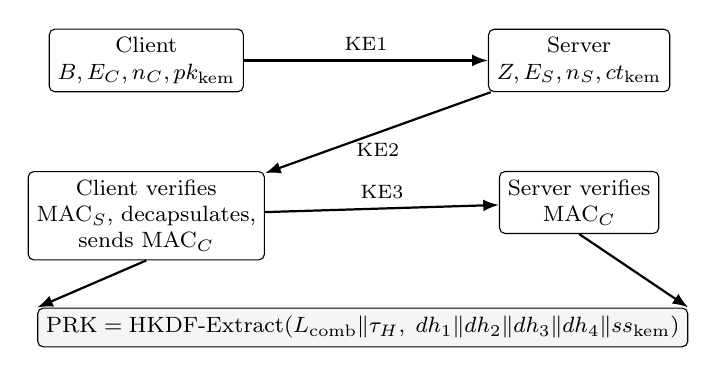
\begin{tikzpicture}[
node distance=0.45cm,
box/.style={draw, rounded corners=2pt, align=center, font=\footnotesize, inner sep=3pt},
arr/.style={-{Latex[length=2mm]}, thick}
]
\node[box] (c1) {Client\\$B,E_C,n_C,pk_{\mathrm{kem}}$};
\node[box, below=1.0cm of c1] (c2) {Client verifies\\MAC$_S$, decapsulates,\\sends MAC$_C$};
\node[box, right=3.1cm of c1] (s1) {Server\\$Z,E_S,n_S,ct_{\mathrm{kem}}$};
\node[box, below=1.0cm of s1] (s2) {Server verifies\\MAC$_C$};
\draw[arr] (c1) -- node[above,font=\scriptsize]{KE1} (s1);
\draw[arr] (s1) -- node[below,font=\scriptsize]{KE2} (c2);
\draw[arr] (c2) -- node[above,font=\scriptsize]{KE3} (s2);
\node[box, fill=black!4, below=1.25cm of $(c2)!0.5!(s2)$, minimum width=6.2cm] (prk)
{$\mathrm{PRK}=\mathrm{HKDF\text{-}Extract}(\Label{comb}\|\tau_H,\;dh_1\|dh_2\|dh_3\|dh_4\|ss_{\mathrm{kem}})$};
\draw[arr] (c2.south) -- (prk.north west);
\draw[arr] (s2.south) -- (prk.north east);
\end{tikzpicture}
\caption{Hybrid PQ-OPAQUE authentication flow. The message pattern is unchanged; final key extraction binds the classical 4DH and ML-KEM layers through the transcript.}
\label{fig:acit-flow}
\end{figure}

\subsection{Message Footprint}

The transport consequence of hybridization is concentrated in KE1 and KE2 because those are the messages that carry the ML-KEM public key and ciphertext. KE3 remains essentially unchanged. This asymmetry is operationally favorable: the protocol does not inflate every step uniformly, but only the two messages in which key-establishment material is naturally exchanged.

\begin{table}[t]
\caption{Authentication message sizes (payload view)}
\label{tab:acit-wire}
\centering
\footnotesize
\begin{tabularx}{\columnwidth}{@{}L{1.0cm}r r Y@{}}
\toprule
Msg & Classical & Hybrid & Main source of growth \\
\midrule
KE1 & 88 B & 1272 B & ML-KEM public key \\
KE2 & 288 B & 1376 B & ML-KEM ciphertext \\
KE3 & 64 B & 64 B & No PQ payload growth \\
\midrule
Total & 440 B & 2712 B & Hybrid AKE material in KE1/KE2 \\
\bottomrule
\end{tabularx}
\end{table}

Table~\ref{tab:acit-wire} shows why the protocol remains deployable despite a non-trivial increase in message footprint. The message pattern is unchanged, and the additional transport burden appears precisely where the protocol already expects public-key material. With the one-byte version prefix carried by each authentication message, the complete wire-format total becomes 2715~bytes. In many deployment settings, this is materially easier to absorb than an additional round trip or a redesign of the authentication choreography.

\section{Security Interpretation and Formal Evidence}

The verification and implementation results form a combined evidence base. ProVerif was used in separate secrecy and authentication models; Tamarin was applied to a surrogate 4DH model that abstracts the classical algebraic core; and the implementation was exercised through reproducible tests and benchmarks. The resulting claim is substantial but delimited: it supports the protocol design and observed implementation behavior, not a universal machine proof of every low-level operation \cite{cremers2012,basin2018}.

\subsection{Formal Reading Discipline}

The manuscript does not collapse symbolic verification, executable tests, and performance measurements into one undifferentiated claim. Each layer answers a different methodological question. ProVerif addresses secrecy and correspondence properties in an unbounded-session symbolic setting \cite{blanchet2016}. Tamarin contributes an event-based account of the hybrid combiner, albeit through a surrogate model of the classical 4DH core rather than a low-level account of every group operation \cite{tamarin2013}. The Rust implementation and its regression tests examine whether the design behaves as intended at the level of wire format, protocol state transitions, and error handling.

This separation is deliberate and methodological. A machine-checked proof of every low-level implementation detail would be stronger, but it is not claimed here. The result is an implementation-backed security argument in which each artifact is assigned an explicit evidentiary role.

\begin{table}[t]
\caption{Security properties and evidence sources}
\label{tab:acit-security-map}
\centering
\footnotesize
\begin{tabularx}{\columnwidth}{@{}L{2.2cm}Y@{}}
\toprule
Property & Main supporting evidence \\
\midrule
Session-key secrecy & ProVerif secrecy model and Tamarin surrogate combiner model. \\
Mutual authentication & ProVerif correspondence queries and protocol regression tests. \\
Offline dictionary scope & OPAQUE structure plus the explicit non-compromise assumption for the server root secret. \\
Hybrid combiner interpretation & Transcript-bound extractor and Tamarin argument for joint weakening of both layers. \\
Wire-level correctness & Rust serialization logic, test vectors, and protocol-state tests. \\
\bottomrule
\end{tabularx}
\end{table}

Table~\ref{tab:acit-security-map} makes the argumentative structure explicit. Hybrid security claims are often weakened less by the protocol idea than by ambiguity over which result supports which statement. The mapping is stated directly.

Concretely, the ProVerif side contributes five checked query families: session-key secrecy, password secrecy, agent-to-relay authentication, relay-to-agent authentication, and injective mutual authentication. The Tamarin side contributes eight verified lemmas covering session-key secrecy, password secrecy, scoped forward secrecy under non-reveal of ephemeral secrets, initiator authenticity, responder authenticity, AND-style combiner interpretation, offline-guessing resistance in the database-compromise model, and executability.

\begin{figure*}[t]
\centering
\includegraphics[width=0.97\textwidth]{fig_2.png}
\caption{Layered evidence structure for Hybrid PQ-OPAQUE. Symbolic and executable artifacts jointly support a scoped implementation-backed claim.}
\label{fig:acit-evidence-stack}
\end{figure*}

Figure~\ref{fig:acit-evidence-stack} summarizes the evidentiary flow. No single artifact is treated as dispositive; each addresses a different methodological question, and the final claim is read only through their combined contribution.

\subsection{Detailed Symbolic Coverage}

\begin{table*}[t]
\caption{Detailed view of supported security properties}
\label{tab:acit-formal-detail}
\centering
\footnotesize
\begin{tabularx}{\textwidth}{@{}L{2.7cm}L{2.5cm}L{2.4cm}Y@{}}
\toprule
Property & ProVerif view & Tamarin view & Interpretation in this paper \\
\midrule
Session-key secrecy & Supported in the secrecy model & Supported in the surrogate hybrid model & Session establishment is consistent with symbolic secrecy in both model families. \\
Mutual authentication & Supported by correspondence queries & Indirectly supported through event discipline & The protocol completion path matches the intended peer agreement story. \\
Offline dictionary resistance & Not modeled as unrestricted server compromise & Scoped to database compromise without root-secret leakage & The claim is limited to the standard OPAQUE-style server-record boundary. \\
Scoped forward secrecy & Not established as a full computational theorem & Supported under non-reveal of ephemeral secrets & The paper claims only the symbolic post-session protection captured by the surrogate model and does not assert a complete post-quantum forward-secrecy proof. \\
Hybrid combiner interpretation & Reflected through transcript-bound secrecy & Central result of the surrogate model & The final extractor is read as requiring joint weakening of both layers in the adopted model. \\
\bottomrule
\end{tabularx}
\end{table*}

Table~\ref{tab:acit-formal-detail} addresses a recurring weakness in hybrid papers: models are presented without a precise statement of what they do and do not support. Here the evidence is partitioned explicitly, and each claim is tied to a specific supporting artifact.

\begin{table*}[t]
\caption{Comparison with canonical 3DH-OPAQUE and supporting evidence}
\label{tab:acit-comparison}
\centering
\footnotesize
\begin{tabularx}{\textwidth}{@{}L{3.0cm}L{3.0cm}L{3.1cm}Y@{}}
\toprule
Aspect & Canonical 3DH-OPAQUE & Hybrid PQ-OPAQUE & Interpretation \\
\midrule
Round complexity & 3 messages, 1.5 rounds & 3 messages, 1.5 rounds & The interaction pattern is preserved. \\
Key schedule input & Classical 3DH material & 4DH material + ML-KEM secret & The final extractor binds both layers through the transcript. \\
Honest-party cost & Baseline AKE cost & $+1$ DH + KEM + $O(1)$ & The additional cost is additive rather than structural. \\
Communication footprint & Baseline handshake size & $+2272$ payload bytes; 2715~B total wire format & The dominant deployment trade-off moves to transport overhead. \\
Compromise condition & Classical layer failure & Joint weakening of classical and PQ layers in the adopted model & The accepted model yields a stricter recovery condition for final key material. \\
Symbolic evidence & Classical OPAQUE literature & ProVerif 5/5 queries; Tamarin 8/8 lemmas & Evidence is multi-source and explicitly scoped. \\
Implementation evidence & Often omitted in prior PAKE papers & 155 passing tests, reproducible Rust artifact & The paper argues from code, models, and measurements together. \\
\bottomrule
\end{tabularx}
\end{table*}

The main formal consequence of the construction is not a new asymptotic security notion, but a different structure of extractor input under an unchanged operational protocol shape. In canonical 3DH-OPAQUE, the authenticated key exchange depends entirely on classical material. Here, the pseudorandom key in \eqref{eq:hybrid-prk-acit} is bound simultaneously to the classical 4DH layer, the post-quantum KEM secret, and the extended transcript. That change justifies the central comparative statement: under the adopted model, final key recovery requires a materially stronger failure story than in the single-layer classical baseline.

\section{Implementation and Experimental Methodology}

The implementation is reported as a reproducible Rust artifact rather than as pseudocode alone. That choice is methodologically necessary for a hybrid augmented PAKE because many deployment-relevant defects are not mathematical: message framing, state-machine drift between parties, incorrect handling of version markers, unsafe cross-language boundaries, or failure to erase ephemeral material after key derivation. Any deployment-oriented claim that omits these layers leaves too much of the protocol surface unexamined.

The implementation architecture is layered. A cryptographic core provides protocol serialization, transcript processing, and key-derivation logic. Client and server protocol contours build on that core. A narrow FFI boundary is used only where low-level interoperability is required. This is not a machine proof of implementation security, but it reduces the number of points at which memory-management defects or inconsistent API semantics can distort the cryptographic design.

\subsection{Artifact Footprint}

\begin{table*}[t]
\caption{Size and composition of the research artifact}
\label{tab:acit-codebase}
\centering
\footnotesize
\begin{tabularx}{\textwidth}{@{}L{3.2cm}L{3.0cm}rY@{}}
\toprule
Component & Role & Lines & Why it matters \\
\midrule
Cryptographic core & Key derivation, transcript processing, serialization & 1509 & Encodes the protocol logic that the paper argues about. \\
Client contour & Initiator-side protocol state machine & 899 & Shows the design is executable beyond pseudocode. \\
Server contour & Responder-side protocol logic & 907 & Captures the real server-side cost path and message handling. \\
FFI layer & Cross-language boundary and exported interface & 2020 & Makes API behavior and boundary safety part of the artifact story. \\
Tests & Regression, protocol, and interface checks & 3961 & Demonstrates that the work is reproducible and not merely descriptive. \\
Formal models & ProVerif and Tamarin material & 1806 & Grounds the scoped formal claims in executable symbolic artifacts. \\
\bottomrule
\end{tabularx}
\end{table*}

The size of the artifact in Table~\ref{tab:acit-codebase} is not reported for its own sake. It explains why the argument relies on layered evidence. A hybrid augmented PAKE simultaneously touches cryptographic routines, protocol choreography, boundary interfaces, and evaluation scripts. Reporting only formal models or only benchmark numbers would conceal that breadth.

\subsection{Memory Safety and Secret Lifecycle}

For a password-authenticated protocol, implementation quality is not determined solely by which primitives are invoked. It also depends on how long sensitive values remain live in memory, whether protocol state can be reused incorrectly, and whether low-level interfaces permit accidental exposure of partially derived secrets. The Rust implementation therefore treats secret lifecycle as a first-class systems property rather than as an afterthought.

Concretely, the initiator path stores DH terms, transcript buffers, PRK material, and the decapsulated ML-KEM secret in zeroizing wrappers, while the responder path explicitly invokes zeroization on classical IKM, MAC inputs, transcript hashes, DH outputs, KEM shared secrets, and retained state on completion, expiry, or authentication failure. At the FFI boundary, handle-owned protocol state is zeroized on drop, and responder-expiry tests assert that private state is cleared after invalidation. These mechanisms do not amount to a full side-channel or compiler-interference proof, but they do define concrete erasure boundaries inside the artifact rather than leaving secret lifecycle as an implicit assumption.

\begin{table}[t]
\caption{Reproducible artifact layers}
\label{tab:acit-artifacts}
\centering
\footnotesize
\begin{tabularx}{\columnwidth}{@{}L{2.2cm}Y@{}}
\toprule
Artifact layer & Role in the evaluation \\
\midrule
Rust implementation & Executable realization of the protocol, wire format, and key schedule. \\
Protocol tests & Regression protection for message sequencing, version checks, and error handling. \\
Formal models & Symbolic support for secrecy, authentication, and hybrid-combiner interpretation. \\
Benchmarks & Reproducible timing data for micro-operations and end-to-end protocol paths. \\
\bottomrule
\end{tabularx}
\end{table}

The benchmarking methodology also requires explicit scope. Measurements were taken on Apple M1 Pro in optimized single-process runs under Criterion. Criterion reports bootstrap estimates of the mean and the 95\% confidence interval; these values should be read as reproducible platform-specific estimates, not as universal constants. Their value lies in the relative ordering of costs: whether the post-quantum layer is dominant, whether the server-side path remains sub-millisecond, and whether the latency bottleneck remains password hardening. Microbenchmarks and protocol-path benchmarks were collected in separate Criterion scenarios, so the reported means are comparable as profiles rather than as additive components of a single timing equation.

The broader reproducibility point is that no single artifact type is sufficient. A symbolic model can succeed while a wire-format implementation still fails; a benchmark can look favorable while the protocol state machine remains fragile; and a clean code base can still overclaim security if its formal scope is unclear. The artifact stack is therefore designed so that the layers reinforce one another rather than substitute for one another.

\section{Quantitative Results}

The measurements support a conservative deployment interpretation. On Apple M1 Pro, the full ML-KEM-768 round costs 122.01~$\mu$s with a 95\% confidence interval of [119.32; 126.96], while isolated server-side KE2 generation remains in the few-hundred-microsecond range. The end-to-end authentication profile is 481.43~ms [471.73; 495.25], but this latency is dominated by Argon2id \cite{argon2rfc2021} rather than by the post-quantum reinforcement itself. Outside password hardening, the post-quantum addition contributes 159.3~$\mu$s of extra computation.

\subsection{Selected Microbenchmarks}

\begin{table}[t]
\caption{Selected microbenchmark results}
\label{tab:acit-microbench}
\centering
\scriptsize
\begin{tabularx}{\columnwidth}{@{}L{1.6cm}L{1.45cm}rY@{}}
\toprule
Primitive & Operation & Mean time & 95\% CI \\
\midrule
Ristretto255 & single DH & 46.41~$\mu$s & [45.94; 46.98] \\
Ristretto255 & 4DH aggregate & $\approx 164$~$\mu$s & [$\approx$162; $\approx$167] \\
ML-KEM-768 & key generation & 41.05~$\mu$s & [40.69; 41.68] \\
ML-KEM-768 & encapsulation & 33.62~$\mu$s & [32.89; 34.95] \\
ML-KEM-768 & decapsulation & 38.55~$\mu$s & [37.65; 40.11] \\
ML-KEM-768 & full round & 122.01~$\mu$s & [119.32; 126.96] \\
Argon2id & moderate profile & 510.86~ms & [490.31; 533.80] \\
\bottomrule
\end{tabularx}
\end{table}

Table~\ref{tab:acit-microbench} reports the central performance result: the hybrid key-establishment layer remains in the microsecond regime, whereas Argon2id remains in the millisecond regime. The post-quantum cost is therefore additive rather than transformative. The protocol becomes larger on the wire and moderately heavier in the AKE path, but it does not change the dominant latency source.

\begin{table}[t]
\caption{Selected headline metrics across benchmark families}
\label{tab:acit-metrics}
\centering
\footnotesize
\begin{tabularx}{\columnwidth}{@{}L{2.4cm}Y@{}}
\toprule
Metric & Value and interpretation \\
\midrule
Full ML-KEM round & 122.01~$\mu$s [119.32; 126.96] on Apple M1 Pro. \\
Isolated responder core & KE2 cryptographic core completes in 254.26~$\mu$s in the isolated responder benchmark. \\
End-to-end authentication & 481.43~ms [471.73; 495.25], dominated by Argon2id rather than PQ AKE work. \\
Post-quantum AKE delta & 159.3~$\mu$s beyond the password-hardening step. \\
Handshake size & 2715~bytes total on the wire, including 2272~bytes of hybrid payload expansion. \\
Artifact evidence & 155 passing tests; ProVerif 5/5 queries; Tamarin 8/8 lemmas. \\
\bottomrule
\end{tabularx}
\end{table}

Table~\ref{tab:acit-metrics} isolates the costs that matter operationally. The end-to-end figure should not be read as post-quantum cryptographic slowdown; the dominant latency source remains password hardening, while the hybrid authenticated key exchange adds only a small amount of extra work in absolute terms. The isolated Argon2id and KE2 measurements characterize where cost resides, not a strict arithmetic decomposition across benchmark harnesses.

\subsection{Protocol-Path Measurements}

\begin{table}[t]
\caption{Protocol-level benchmark scenarios}
\label{tab:acit-protocol}
\centering
\scriptsize
\begin{tabularx}{\columnwidth}{@{}L{1.35cm}L{1.75cm}rY@{}}
\toprule
Phase & Scenario & Mean time & 95\% CI \\
\midrule
Reg. & request & 72.46~$\mu$s & [72.15; 72.77] \\
Reg. & response & 45.92~$\mu$s & [45.72; 46.16] \\
Reg. & completion & 479.58~ms & [472.11; 487.75] \\
Auth. & KE1 generation & 118.83~$\mu$s & [116.59; 121.76] \\
Auth. & KE2 generation & 297.03~$\mu$s & [294.81; 299.69] \\
Auth. & KE3 at initiator & 492.34~ms & [478.95; 509.96] \\
Full & full cycle & 481.43~ms & [471.73; 495.25] \\
\bottomrule
\end{tabularx}
\end{table}

The protocol-path measurements show where the engineering budget is spent. Responder-side cryptographic work remains sub-millisecond, which is compatible with server-side scalability. The initiator-side completion path is slower for the same reason as in the classical setting: password hardening dominates the cost profile. KE3 generation and the complete authentication cycle were measured in separate Criterion scenarios with different state-initialization paths, so their means are not additive and the full-cycle mean may fall slightly below the isolated phase mean while the 95\% confidence intervals still overlap. The post-quantum addition changes the composition of authentication only marginally.

This lets us state the main comparative result compactly:
\begin{equation}
\begin{aligned}
C_{\mathrm{hyb}} &= C_{\mathrm{opq}} + C_{\mathrm{1DH}} + C_{\mathrm{KEM}} + O(1), \\
\Delta W_{\mathrm{payload}} &= 2272~\mathrm{bytes}.
\end{aligned}
\label{eq:complexity-acit}
\end{equation}
Equation \eqref{eq:complexity-acit} captures the central systems point: the protocol does not move to a new interaction class, yet it materially hardens the compromise structure in the adopted hybrid model.

Since isolated KE2 generation remains in the few-hundred-microsecond range, the responder path remains compatible with high authentication throughput on commodity hardware. The construction is therefore persuasive not only in end-user latency terms but also in server-provisioning terms, where fixed-round interaction and bounded work per authentication are both valuable.

The security interpretation remains conservative. Claims about offline dictionary resistance are limited to the case in which the attacker compromises the database record but not the root secret from which account-specific OPRF keys are derived. Likewise, the Tamarin result is a surrogate symbolic argument for the hybrid combiner rather than a complete computational proof for every algebraic detail of Ristretto255.

\subsection{Threats to Validity}

\begin{table}[t]
\caption{Scope of claims and supporting evidence}
\label{tab:acit-scope}
\centering
\footnotesize
\begin{tabularx}{\columnwidth}{@{}L{2.1cm}Y@{}}
\toprule
Claim dimension & Covered scope and explicit limit \\
\midrule
Secrecy and authentication & Supported by symbolic models; not presented as a tight computational reduction. \\
Password protection & Interpreted for database-record compromise without compromise of the server root secret. \\
Performance profile & Reproducible on Apple M1 Pro; not claimed as a universal cross-platform bound. \\
Deployment claim & Fixed-round interaction is preserved; transport overhead still has to be absorbed operationally. \\
\bottomrule
\end{tabularx}
\end{table}

Table~\ref{tab:acit-scope} summarizes the intended reading discipline. The objective is not to overstate the result, but to state the claim precisely: the work contributes an implementation-backed hybridization pattern whose security interpretation is meaningful for systems design while remaining explicit about the abstractions used in symbolic verification and benchmarking.

These limitations also strengthen the credibility of the result. A weaker formulation would claim end-to-end post-quantum security for the entire authentication stack. The claim advanced here is narrower and more defensible: a post-quantum reinforcement of the OPAQUE key-establishment layer that preserves the interaction pattern, quantifies the deployment cost, and states its assumptions directly.

\section{Deployment Considerations}

The deployment value of a hybrid augmented PAKE depends on more than security semantics. Operators need to know whether the protocol fits existing authentication surfaces, whether server provisioning changes materially, and whether migration can proceed incrementally. The answer here is conservative: the message pattern is preserved, the password-hardening stage remains familiar, and the additional post-quantum cost is concentrated in the authenticated key-exchange portion rather than across the entire account workflow.

\begin{table}[t]
\caption{Operational implications of the hybrid design}
\label{tab:acit-deployment}
\centering
\footnotesize
\begin{tabularx}{\columnwidth}{@{}L{2.1cm}Y@{}}
\toprule
Operational concern & Interpretation for Hybrid PQ-OPAQUE \\
\midrule
Round trips & No new round trip is introduced. \\
Server hot path & KE2 remains sub-millisecond in isolation. \\
Client latency & Still dominated by Argon2id rather than by the post-quantum layer. \\
Transport budget & Larger KE1/KE2 messages must be absorbed by the surrounding system. \\
Migration path & The protocol can be introduced as a reinforcement of OPAQUE, not as a replacement of password authentication logic. \\
\bottomrule
\end{tabularx}
\end{table}

Table~\ref{tab:acit-deployment} shows why the proposal is operationally viable in real systems. The most difficult operational changes in authentication usually arise when a protocol adds a round trip, changes the server-side account model, or imposes substantial cryptographic cost on the hot path. None of those occurs here. The main change is the transport footprint of the first two messages, which is a materially simpler engineering problem than redesigning the authentication choreography.

There is also a sequencing argument for migration. Organizations that already depend on password authentication rarely replace the entire stack in one step. They need transitional designs that can be justified to engineering teams, product owners, and security review boards. A fixed-round hybrid OPAQUE variant fits that setting because the migration path is incremental: preserve the interaction shape, preserve the password-hardening boundary, add a post-quantum layer to the key-establishment core, and validate the result through code and measurements.

The contribution therefore concerns deployment posture as much as protocol composition. The quantitative results show that the cost of hybridization is bounded. The formal results show that the stronger compromise condition is not merely heuristic. The implementation artifact shows that the design withstands serialization, interface boundaries, and regression testing.

\section{Discussion and Conclusion}

Hybrid PQ-OPAQUE shows that post-quantum reinforcement of augmented PAKE can be achieved without increasing round complexity. In the measured implementation, the dominant deployment cost is transport overhead rather than CPU cost: Argon2id remains the latency bottleneck, while the additional authenticated key-exchange work is additive and sub-millisecond. The construction therefore preserves the operational profile of OPAQUE while introducing a bounded and quantified migration cost.

The main scientific point is comparative. Relative to canonical 3DH-OPAQUE, the construction preserves fixed-round interaction, increases honest-party cost only additively, and strengthens the condition for final key recovery in the adopted model. The value of the result lies less in a new asymptotic abstraction than in demonstrating that a strong augmented-PAKE baseline can be hybridized without forfeiting deployment realism.

The claim remains deliberately scoped. It rests on a layered evidence base spanning symbolic analysis, executable code, regression tests, and measurements, and it should be read as an implementation-backed protocol-engineering result rather than as a full computational proof. Under that reading, Hybrid PQ-OPAQUE provides a reproducible and quantitatively characterized fixed-round migration pattern for augmented PAKE.

Natural next steps are equally concrete: a tighter computational treatment of the hybrid combiner and its forward-secrecy boundary, cross-platform measurements under varied Argon2id profiles and transport settings, and broader interoperability checks across independently implemented endpoints. Each would narrow a specific current limitation without altering the central fixed-round engineering result established here.

% \clearpage
% \onecolumn
\section*{ACKNOWLEDGMENT}
OpenAI Codex was used during manuscript preparation to assist with English-language drafting, stylistic revision, and \LaTeX{} editing in portions of the abstract, introduction, discussion, conclusion, and related connective prose. The system was not used as an authoritative source for technical claims. All protocol descriptions, equations, references, tables, implementation details, and experimental results were independently reviewed, verified, and approved by the author.

\begin{thebibliography}{23}

\bibitem{en18071823}
S.~Svystun, L.~Scislo, M.~Pawlik, O.~Melnychenko, P.~Radiuk, O.~Savenko, and A.~Sachenko, ``DyTAM: Accelerating wind turbine inspections with dynamic UAV trajectory adaptation,'' \emph{Energies}, vol.~18, no.~7, p.~1823, 2025. doi:~\url{https://doi.org/10.3390/en18071823}.

\bibitem{Svystun_Melnychenko_Radiuk_Savenko_Sachenko_Lysyi_2024}
S.~Svystun, O.~Melnychenko, P.~Radiuk, O.~Savenko, A.~Sachenko, and A.~Lysyi, ``Thermal and RGB images work better together in wind turbine damage detection,'' \emph{International Journal of Computing}, vol.~23, no.~4, pp.~526--535, Dec. 2024. doi:~\url{https://doi.org/10.47839/ijc.23.4.3752}.

\bibitem{reksreks.2025.2.06}
A.~Lysyi, A.~Sachenko, P.~Radiuk, M.~Lysyi, O.~Melnychenko, O.~Ishchuk, and O.~Savenko, ``Enhanced fire hazard detection in solar power plants: an integrated UAV, AI, and SCADA-based approach,'' \emph{Radioelectronic and Computer Systems}, no.~2, pp.~99--117, 2025. doi:~\url{https://doi.org/10.32620/reks.2025.2.06}.

\bibitem{jarecki2018}
S.~Jarecki, H.~Krawczyk, and J.~Xu, ``OPAQUE: An asymmetric PAKE protocol secure against pre-computation attacks,'' in \emph{EUROCRYPT 2018}, LNCS~10822, pp.~456--486, 2018. doi:~\url{https://doi.org/10.1007/978-3-319-78372-7_15}.

\bibitem{ietf-opaque}
D.~Bourdrez, H.~Krawczyk, K.~Lewi, and C.~A.~Wood, ``The OPAQUE augmented password-authenticated key exchange (aPAKE) protocol,'' RFC~9807, Jul.~2025. Available:~\url{https://www.rfc-editor.org/info/rfc9807}.

\bibitem{ladd2023}
W.~Ladd, ``SPAKE2, a password-authenticated key exchange,'' RFC~9382, Sep.~2023. Available:~\url{https://www.rfc-editor.org/info/rfc9382}.

\bibitem{spake2plus2023}
T.~Taubert and C.~A.~Wood, ``SPAKE2+, an augmented password-authenticated key exchange (PAKE) protocol,'' RFC~9383, Sep.~2023. Available:~\url{https://www.rfc-editor.org/info/rfc9383}.

\bibitem{mosca2018}
M.~Mosca, ``Cybersecurity in an Era with Quantum Computers: Will We Be Ready?,'' \emph{IEEE Security \& Privacy}, vol.~16, no.~5, pp.~38--41, Sep./Oct.~2018. doi: 10.1109/MSP.2018.3761723.

\bibitem{shor1994}
P.~W.~Shor, ``Algorithms for quantum computation: discrete logarithms and factoring,'' in \emph{Proceedings of the 35th Annual Symposium on Foundations of Computer Science}, 1994, pp.~124--134. Expanded version available:~\url{https://arxiv.org/abs/quant-ph/9508027}.

\bibitem{bernstein2017}
D.~J.~Bernstein and T.~Lange, ``Post-quantum cryptography,'' \emph{Nature}, vol.~549, no.~7671, pp.~188--194, 2017. doi:~\url{https://doi.org/10.1038/nature23461}.

\bibitem{roetteler2017}
M.~Roetteler, M.~Naehrig, K.~M.~Svore, and K.~Lauter, ``Quantum resource estimates for computing elliptic curve discrete logarithms,'' in \emph{ASIACRYPT 2017}, LNCS~10625, pp.~241--270, 2017. doi:~\url{https://doi.org/10.1007/978-3-319-70697-9_9}.

\bibitem{babbush2026}
R.~Babbush, A.~Zalcman, C.~Gidney, M.~Broughton, T.~Khattar,
H.~Neven, T.~Bergamaschi, J.~Drake, and D.~Boneh,
``Securing elliptic curve cryptocurrencies against quantum vulnerabilities:
Resource estimates and mitigations,'' arXiv:2603.28846, Mar.~2026.
doi:~\url{https://doi.org/10.48550/arXiv.2603.28846}.

\bibitem{fips203}
National Institute of Standards and Technology, ``Module-Lattice-Based Key-Encapsulation Mechanism Standard,'' FIPS~203, Aug.~2024. doi:~\url{https://doi.org/10.6028/NIST.FIPS.203}.

\bibitem{fips204}
National Institute of Standards and Technology, ``Module-Lattice-Based Digital Signature Standard,'' FIPS~204, Aug.~2024. doi:~\url{https://doi.org/10.6028/NIST.FIPS.204}.

\bibitem{canetti2001}
R.~Canetti, ``Universally composable security: A new paradigm for cryptographic protocols,'' in \emph{Proceedings of the 42nd IEEE Symposium on Foundations of Computer Science}, 2001, pp.~136--145. Full version available:~\url{https://eprint.iacr.org/2000/067}.

\bibitem{tlshybrid2025}
D.~Stebila, S.~Fluhrer, and S.~Gueron, ``Hybrid key exchange in TLS 1.3,'' Internet-Draft draft-ietf-tls-hybrid-design-16, Sep.~2025. Work in progress. Available:~\url{https://datatracker.ietf.org/doc/draft-ietf-tls-hybrid-design/}.

\bibitem{devalence2024}
H.~de~Valence, J.~Grigg, M.~Hamburg, I.~Lovecruft, G.~Tankersley, and F.~Valsorda, ``The ristretto255 and decaf448 groups,'' RFC~9496, Dec.~2023. Available:~\url{https://www.rfc-editor.org/info/rfc9496}.

\bibitem{krawczyk2010}
H.~Krawczyk and P.~Eronen, ``HMAC-based extract-and-expand key derivation function (HKDF),'' RFC~5869, May~2010. Available:~\url{https://www.rfc-editor.org/info/rfc5869}.

\bibitem{cremers2012}
C.~Cremers and S.~Mauw, \emph{Operational Semantics and Verification of Security Protocols}. Springer, 2012. doi:~\url{https://doi.org/10.1007/978-3-540-78636-8}.

\bibitem{basin2018}
D.~Basin, C.~Cremers, and C.~Meadows, ``Model checking security protocols,'' in \emph{Handbook of Model Checking}, Springer, 2018, pp.~727--762. doi:~\url{https://doi.org/10.1007/978-3-319-10575-8_22}.

\bibitem{blanchet2016}
B.~Blanchet, ``Modeling and verifying security protocols with the applied pi calculus and ProVerif,'' \emph{Foundations and Trends in Privacy and Security}, vol.~1, nos.~1--2, pp.~1--135, 2016. Available:~\url{https://bblanche.gitlabpages.inria.fr/publications/BlanchetFnTPS16.pdf}.

\bibitem{tamarin2013}
S.~Meier, B.~Schmidt, C.~Cremers, and D.~Basin, ``The TAMARIN prover for the symbolic analysis of security protocols,'' in \emph{CAV 2013}, LNCS~8044, pp.~696--701, 2013. doi:~\url{https://doi.org/10.1007/978-3-642-39799-8_48}.

\bibitem{argon2rfc2021}
A.~Biryukov, D.~Dinu, D.~Khovratovich, and S.~Josefsson, ``Argon2 memory-hard function for password hashing and proof-of-work applications,'' RFC~9106, Sep.~2021. Available:~\url{https://www.rfc-editor.org/info/rfc9106}.

\end{thebibliography}

% Just in case for the future
% \begin{IEEEbiography}[{\includegraphics[width=1in,height=1.25in,clip,keepaspectratio]{photos/2_Melnychenko.jpg}}]{Oleksandr Melnychenko} Ph.D. in Computer Science, Senior Lecturer at the Department of Computer Engineering and Information Systems, Khmelnytskyi National University, Khmelnytskyi, Ukraine. His research interests encompass distributed multi-agent systems, post-quantum cryptography, and symbolic verification.
% \end{IEEEbiography}

\end{document}
